% TODO:
%   - Kijk na of titels in header overflowen
% ----------  
% Questions:
%   - XXX

% Kijk naar wat Arnau review zegt over "minimal reporting"

\part{Development of motor imagery EEG classifiers}
\label{part:development}

\chapter{EEG-based offline classification system for motor imagery tasks}
\label{ch:offline_bci_system}

% ---------------------------------------------- 
% INTRODUCTION
% ---------------------------------------------- 
\section{Introduction to this chapter}
\label{sec:offline_bci_system_introduction}
% NOTE: "Introduction" exists in each chapter and gives a short intro to the chapter + what can be expected in the chapter

This Chapter discusses the seven different \gls{eeg} based \gls{mi} classification pipelines that were considered in this master thesis.
In particular, two traditional two-step \gls{ml} approaches were considered, both based on the \gls{csp} feature extraction technique.
These two approaches differ by the frequency filter they use in their preprocessing step, where one is fixed throughout all experiments and the other is configured using hyperparameter tuning.
The proven to be better performing extension to \gls{csp}, \gls{fbcsp}, is also discussed but not considered for the experiments in this master thesis.

The other five classification pipelines that were considered in this master thesis are one-step \gls{dl} approaches, as this master thesis focuses primarily on these kinds of approaches.
First, three literature proposed state-of-the-art \gls{cnn}-based approaches are discussed: EEGNet, Deep\-Conv\-Net and ShallowConvNet.
Both their architectural design and some implementation details are discussed.
The visualisation possibilities of these \gls{cnn}-based \gls{eeg} classification algorithms are also addressed.

The final two \gls{dl} classification pipelines that were considered in this master thesis are an extension to EEGNet proposed by this master thesis.
Both of these extensions aim to provide additional memory to EEGNet by incorporating \gls{lstm} functionality. 
One reuses all components of the EEGNet architectural design but adds a tunable \gls{lstm} layer right before the softmax layer.
The other approach only reuses part of the original EEGNet architectural design and makes use of a convolutional \gls{lstm} layer.
Again, some of the implementation details are also addressed.

All of the implemented pipelines together with the performed experiments and saved results are available on the GitHub page of this master thesis \citep{github_project}.
The state-of-the-art literature proposed \gls{cnn}-based \gls{dl} models are a modified version of the Keras reimplementation provided by \citet{arl_eegmodels} and are made available in the utillity file: $\texttt{EEGModels.py}$.
The EEGnet extensions are provided in the utility file: $\texttt{EEGNet\_with\_lstm.py}$.
A custom filter that is hyperparameter tunable with \gls{sklearn} has also been made and is available in the utility file $\texttt{custom\_sklearn\_components.py}$.
More general Keras and TensorFlow tools are also made available in a separate utility file: $\texttt{TF\_tools.py}$.
All these utility files can easily be imported and have the required inline documentation to make reusing them easy.

% ---------------------------------------------- 
% Two-step ML approaches
% ---------------------------------------------- 
\section{CSP-based two-step ML approaches}
\label{sec:offline_bci_system_two_step_ml}

As discussed, the focus of this master thesis lies on one-step \gls{dl} \gls{mi} \gls{eeg} classification pipelines, as these are most widely used in \gls{bc} systems according to \citet{bci_review_arnau}.
However, considering the significant role \gls{csp} played in allowing \gls{ml} approaches to effictively learn from \gls{eeg} data, accelerating the field of \gls{bci} research, this master thesis also considers two traditional two-step \gls{mi} \gls{eeg} \gls{ml} classification approaches based on \gls{csp}.
The architectural design of both of these pipelines is discussed in what follows.

It is noted that since the introduction of \gls{csp} by \citet{first_csp}, many extensions have been proposed that have proven to be far superior to this original version \citep{eeg_model_fbcsp, bci_book_csp_extension}.
As such, the results obtained from these two regular \gls{csp} pipelines discussed in Chapter \ref{ch:evaluation} should not be taken as an indicator of the performance for traditional two-step \gls{mi} \gls{eeg} \gls{ml} classification approaches in general.

% - - - - - - - - - -
% CSP explained
% - - - - - - - - - -

\subsection{The idea behind common spatial pattern(s) (CSP)}
\label{subsec:offline_bci_system_two_step_ml_csp_explained}

Just as \gls{svm} was a classification method originally proposed to solve binary classification tasks (see Section \ref{subsec:processing_signals_ml_and_dl_ml_classifiers}), \gls{csp} was originally proposed to find a spatial filter for feature extraction that leads to optimal variances between two classes of \gls{eeg} data.
The general idea of a spatial filter for feature extraction was already discussed in Section \ref{subsec:processing_signals_general_pipeline_features}.
This is a non-trivial task due to \gls{ers} and \gls{erd} signals, such as \gls{mi}, being time-locked to the event but not phase-locked and them being oscillatory processes.
To achieve an effective optimal variance between two classes of \gls{eeg} data, \gls{csp} has to make some assumptions.
\gls{csp} assumes the frequency band of interest is known, as discussed in Section \ref{subsec:biomedical_signals_working_with_eeg_brain_waves}, this was around 7\gls{hz} to 30\gls{hz} in case of \gls{mi} tasks.
Another assumption that is made is that the time window is known, which is more difficult to ensure as windowing the data around an event in the prediction timeline is not always possible, as further discussed in Section \ref{subsec:processing_signals_general_pipeline_windowing}.
Luckily, \gls{csp} can still work reasonably well even if both frequency band and time window estimations are off.
Besides these assumptions, \gls{csp} also assumes that the band-passed signal is jointly Gaussian within the time window and that there is a difference in the oscillatory signals between both classes.
Both of these assumption hold for most \gls{mi} \gls{eeg} data.

As discussed in Section \ref{subsec:processing_signals_general_pipeline_features}, the goal of a spatial filter is determining an optimal weight matrix $W$ for Equation \ref{eq:processing_signals_spatial_filter}.
In that section, it was also discussed how some data-driven solutions such as \gls{pca} and \gls{ica} do not use the class information, which can have degrading effects.
The goal of \gls{csp} is to find a weight matrix $W$ so that the variance of one signal is minimal, whilst the variance of the other is maximal.
This is shown in Figure \ref{fig:offline_bci_system_csp} where before filtering (Figure \ref{fig:offline_bci_system_csp_pre}) the signals are highly overlapping and though to discriminate, but after using \gls{csp} the signals are far easier to discriminate.

\begin{figure}[t]
    \centering
    \begin{subfigure}{0.45\textwidth}
        \centering
        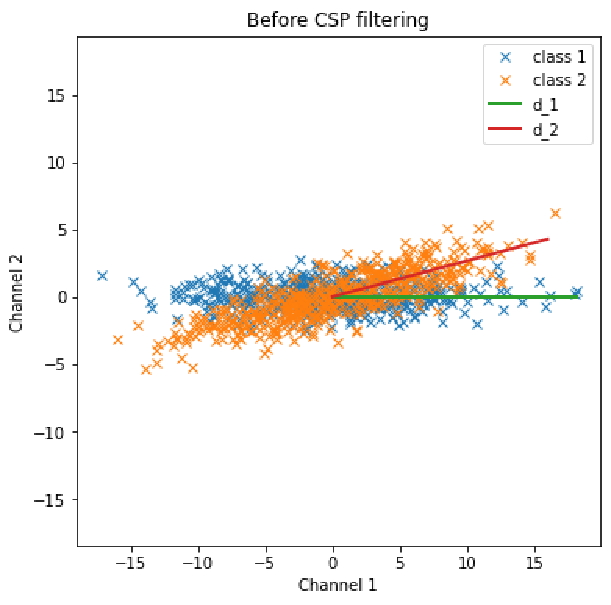
\includegraphics[width=\textwidth]{../images/offline/pre_csp.pdf}
        \captionsetup{width=\linewidth}
        \captionsetup{justification=centering}
        \caption{An arbitrary two-channel signal for two classes before \gls{csp} feature extraction. Free figure by MalcolmSlaney, CC BY-SA 4.0, via Wikimedia Commons.}
        \label{fig:offline_bci_system_csp_pre}
    \end{subfigure}
    \hfill
    \begin{subfigure}{0.45\textwidth}
        \centering
        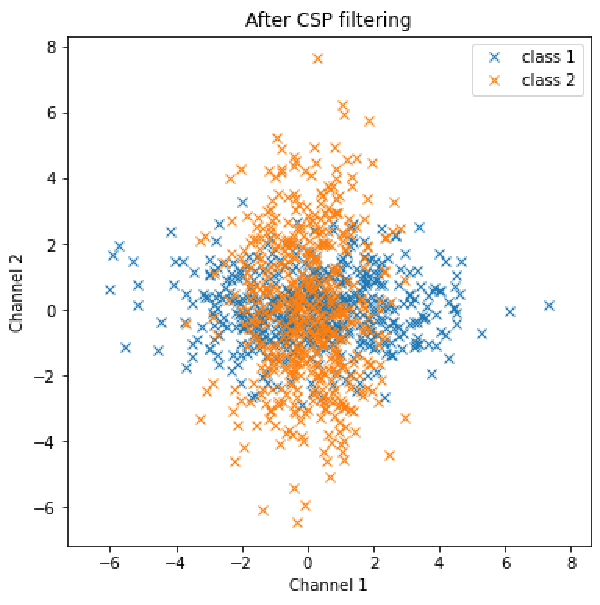
\includegraphics[width=\textwidth]{../images/offline/post_csp.pdf}
        \captionsetup{width=\linewidth}
        \captionsetup{justification=centering}
        \caption{An arbitrary two-channel signal for two classes after \gls{csp} feature extraction. Free figure by MalcolmSlaney, CC BY-SA 4.0, via Wikimedia Commons.}
        \label{fig:offline_bci_system_csp_post}
    \end{subfigure}
    \captionsetup{width=\linewidth}
    \captionsetup{justification=centering}
    \caption{Visualisation of the spatial transformation performed by \gls{csp}.}
    \label{fig:offline_bci_system_csp}
\end{figure}

There are multiple approaches to calculating the optimal weight matrix $W$ based on the optimal variance criteria.
Most commonly are using an optimisation problem, describing it as a generalized Eigenvalue problem and a more geometric approach.
The remainder of this section will discuss the generalized Eigenvalue problem approach.
\Citet{csp_optim_problem} discuss an optimisation approach in more detail, \citet{csp_geometry} does the same for a geometric approach.

The optimal weight matrix $W$ for Equation \ref{eq:processing_signals_spatial_filter} based on the \gls{csp} criteria can be mathematically described as shown in Equation \ref{eq:offline_bci_system_csp_w}.
In this equation, $X_i$ denotes the windows of class $i$ represented as a 2D matrix of $n$ channels by $t_i$ \gls{eeg} measurements per channel.
Due to the jointly Gaussian assumption, the covariance matrix of the signals per class can be easily calculated using Equation \ref{eq:offline_bci_system_csp_cov} where $i$ denotes the class of interest.
From this, the generalized Eigenvalue problem can be created to solve the problem.
Namely, the goal is to find the Eigenvectors $\mathbf{P}$ which contain the Eigenvector of any channel $j$ ($\mathbf{p_j}$) such that Equation \ref{eq:offline_bci_system_csp_solution} holds.
In this Equation, $\mathbf{I}_n$ denotes the identiy matrix for $i$ channels.
This problem can be further reduced to the Eigenvalue decomposition shown in Equation \ref{eq:offline_bci_system_csp_solution_eigen}.
From this, $\mathbf{w}$ can finally be found by taking $\mathbf{w} = \mathbf{p}^T_1$.
\Citet{csp_eigenvals} provides a more detailed explanation of the generalized Eigenvalue problem approach for solving \gls{csp} and some additional steps that help make it more applicable to \gls{bci} settings.

\begin{equation}
    \label{eq:offline_bci_system_csp_w}
    \mathbf{w} = \underset{\mathbf{w}}{\arg\max} \frac{|| \mathbf{w} X_1 ||^2}{|| \mathbf{w} X_2 ||^2}
\end{equation}

\begin{equation}
    \label{eq:offline_bci_system_csp_cov}
    \mathbf{R}_i = \frac{ \mathbf{X}_i \mathbf{X}_i^T }{t_i}
\end{equation}

\begin{equation}
    \label{eq:offline_bci_system_csp_solution}
    \begin{aligned}
        &\mathbf{P}^T \mathbf{R}_1 \mathbf{P} = \mathbf{D}
        \\
        &\text{and}
        \\
        &\mathbf{P}^T \mathbf{R}_2 \mathbf{P} = \mathbf{I}_n
    \end{aligned}
\end{equation}

\begin{equation}
    \label{eq:offline_bci_system_csp_solution_eigen}
    \mathbf{R}^{-1}_2 \mathbf{R}_1 = \mathbf{P} \mathbf{D} \mathbf{P}^{-1}
\end{equation}


% - - - - - - - - - -
% tradtional CSP
% - - - - - - - - - -

\subsection{Traditional CSP with LDA, SVM and RF}
\label{subsec:offline_bci_system_two_step_ml_basic_csp}

\begin{figure}[t]
    \centering
    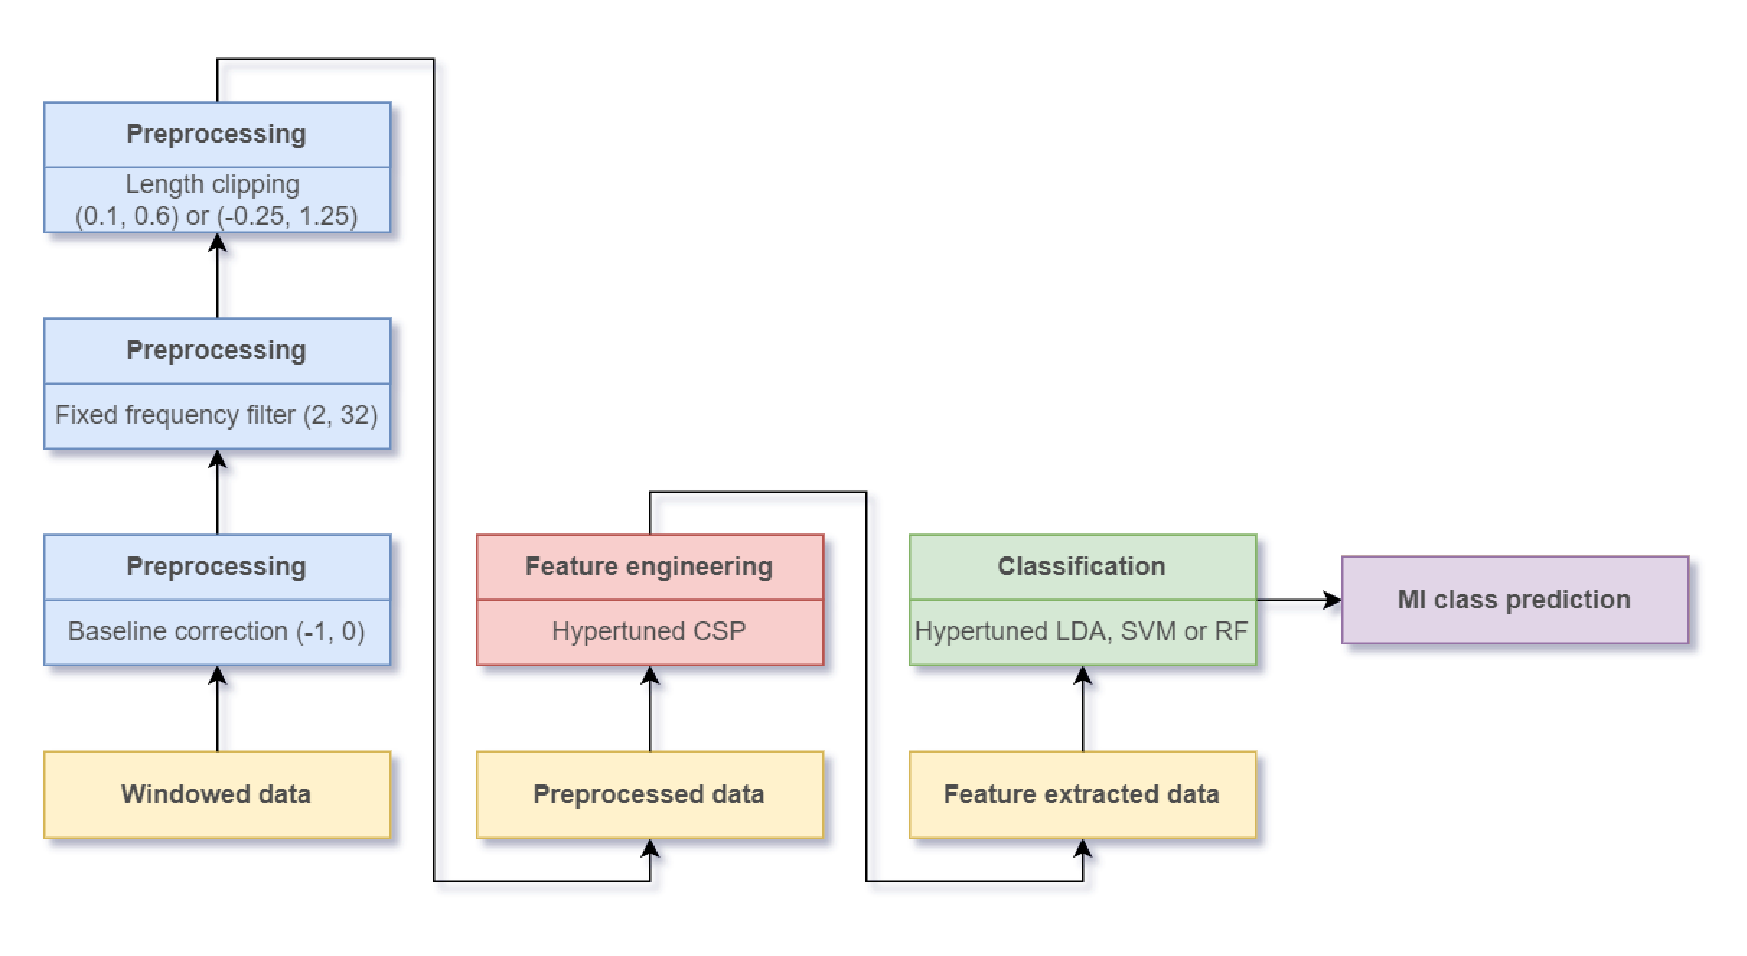
\includegraphics[width=\linewidth]{../images/offline/csp_fixed_filter_pipeline.pdf}
    \captionsetup{width=0.8\linewidth}
    \captionsetup{justification=centering}
    \caption{Visual overview of the pipeline used for \gls{mi} \gls{eeg} classification using the standard \gls{csp} method and multiple traditional two-step \gls{ml} classifiers.}
    \label{fig:offline_bci_system_csp_fixed_filter_pipeline}
\end{figure}

Having explained the idea behind \gls{csp}, the pipelines using \gls{csp} in the experiments of this master thesis can be discussed.
The first pipeline uses the standard \gls{csp} feature extraction method for classifying \gls{mi} \gls{eeg} data in an offline setting and is visualised in Figure \ref{fig:offline_bci_system_csp_fixed_filter_pipeline}.
As discussed further in Section \ref{sec:evaluation_data_source} the used data considers a fixed 3-second window surrounding a known event, including 1 second before the event onset and two seconds after the event onset.
As discussed in Section \ref{subsec:processing_signals_general_pipeline_windowing}, different windowing stragies exist but are not epxlored in this master thesis, in part due to \gls{csp} assuming a known fixed time window as discussed in Section \ref{subsec:offline_bci_system_two_step_ml_csp_explained}.

The windowed data is first preprocessed with multiple preprocessing techniques that were already discussed in Section \ref{subsec:processing_signals_general_pipeline_preprocessing}.
First, the window is baseline correct on one second of data before the event onset.
The resulting data is further preprocessed to only include frequencies between 2\gls{hz} and 32\gls{hz}.
This is done by the use of a \gls{fir} filter design using the Blackman window method.
Whilst Section \ref{subsec:biomedical_signals_working_with_eeg_brain_waves} discussed \gls{mi} is mostly present in the frequency range of 7\gls{hz} to 30\gls{hz}, the boundaries were loosened to account for a fixed approach that is not hyper-tuned on a subject basis and the inclusion of a \textit{neutral} class, which is not a specific \gls{mi} task and most likely has lower frequency brain waves when taking into account the brainwave subdivision given in Table \ref{tab:biomedical_signals_brainwaves}.
Finally, the resulting data is clipped to a 2D matrix (channels x \gls{eeg} measurements) including the samples from either 0.1 seconds after the event onset to 0.6 seconds after the event onset or from 0.25 seconds before the event onset to 1.25 seconds after the event onset, depending on the experiment setup.
It should be noted there is no explicit band-stop filter in place to cancel out the \gls{ac} artefacts discussed in Section \ref{subsec:biomedical_signals_working_with_eeg_artefacts} as the used dataset has already filtered out these frequencies \citep{eeg_data}.

For feature engineering, the multiclass \gls{csp} method described by \citet{used_mc_csp} is used.
The use of a variant is needed as the \gls{csp} method discussed in Section \ref{subsec:offline_bci_system_two_step_ml_csp_explained} only support binary classification where the experiments from this master thesis use three-class \gls{mi} \gls{eeg} data.
The number of \gls{csp} components is hyperparameter tuned based on the possible selection of 2, 3, 4, 6 or 10 components.
This number may seem limited but providing more components will make overfitting more likely and in practice, the differences between six or more \gls{csp} components were found to be minimal after some pilot studies done in the experimental notebooks available on the GitHub repository of this master thesis \citep{github_project}.

For classification, three different classifiers were considered, \gls{lda}, \gls{svm} and \gls{rf}, all three of which were discussed in detail in Section \ref{subsec:processing_signals_ml_and_dl_ml_classifiers}.
As discussed, part of the reason the \gls{lda} classifier is so attractive is due to it not requiring specific hyperparameter tuning.
As such, the \gls{lda} classifier was not hyperparameter tuned in all but a few experiments that validated there was indeed negligible difference when changing the solver and tolerance values from their default parameters.
For the \gls{svm} classifier, the earlier discussed C value for controlling the smoothness of the boundary when using the kernel trick was hyperparameter tuned by trying multiple values between 0.01 and 100.
The kernel was also hyperparameter tuned by trying the \gls{rbf}, sigmoid and linear kernels.
For the \gls{rbf} and sigmoid kernel, the gamma parameter denoting the kernel coefficient was also hyper-tuned on values between 0.001 and 10, including some calculated values provided by \gls{sklearn}.
Finally, the \gls{rf} classifier was hyperparameter tuned for the number of decision trees (values between 10 and 500) in its ensemble as well as the maximum depth (3, 10 or no limit), minimal sample split (2, 5 or 10) and features (different percentual proportion including no limit) to be used by each of those decision trees.

The used preprocessing techniques and \gls{csp} methods are supplied by the Python MNE library \citep{mne}.
The traditional two-step \gls{ml} classifiers are provided by the \gls{sklearn} library from which the hyperparameter tuning functionalities were also used to hyperparameter tune the required components of this pipeline \citep{sklearn}.

% - - - - - - - - - -
% issue basic CSP
% - - - - - - - - - -

\subsection{The issue with a traditional CSP approach}
\label{subsec:offline_bci_system_two_step_ml_basic_csp_issue}
It has been discussed that in the classification of \gls{mi} \gls{eeg} data using \gls{csp} feature extraction paired with almost any classifier, even simple one such as \gls{lda}, can produce pleasant results for some experimental settings.
However, \gls{csp} in itself is a limited feature extraction method compared to the proposed extensions that have far outperformed it \citep{eeg_model_fbcsp, bci_book_csp_extension, four_class_mi_CSP_good, eeg_mi_model_lda_csp}.
To understand the intuitive reasoning behind most \gls{csp} extension, a different pipeline is configured where the fixed frequency filtering in the preprocessing step of the pipeline shown in Figure \ref{fig:offline_bci_system_csp_fixed_filter_pipeline} is now hyperparameter tunable.
Practically, this is done by providing an equal filtertering strategy as the one described in Section \ref{subsec:offline_bci_system_two_step_ml_basic_csp} through a \gls{sklearn} transformer.
For this custom \gls{sklearn} transformer provided in the $\texttt{custom\_sklearn\_components.py}$ utility file of this GitHub project, the lower bound and upper bound can be configured \citep{github_project}.
Being a \gls{sklearn} transformer, it can be used in the same hyperparameter tuning strategy as described in Section \ref{subsec:offline_bci_system_two_step_ml_basic_csp} to find optimal lower bound values and upper bound values.

From the results of these experiments, which are further discussed in Chapter \ref{ch:evaluation}, it becomes clear that the performance of \gls{csp} is heavily dependent on the used frequency filtering.
Accuracy for the worst found parameters and best parameters in 4-fold cross-validation ranged from 30\% to 75\% in an intrasession testing setup.
This huge fluctuation in performance follows from the assumption of a know frequency band that \gls{csp} makes as discussed in Section \ref{subsec:offline_bci_system_two_step_ml_csp_explained}.
The best found frequencies were also subject dependent, as Section \ref{subsec:biomedical_signals_working_with_eeg_brain_waves} already suggested.
Whilst incorporating this hyperparameter tuning as a training procedure in the \gls{csp} approach would already increase the performance of \gls{csp} by automating the finding of the best frequency range for a subject, even better solutions have been proposed.
These follow mainly from an equal intuitive idea of learning the frequency band(s) of interest.
The next session will discuss the commonly used \gls{fbcsp} extension of \gls{csp}.


% - - - - - - - - - -
% improving traditional CSP
% - - - - - - - - - -

\subsection{Improving traditional CSP with FBCSP}
\label{subsec:offline_bci_system_two_step_ml_basic_csp_improving}

\begin{figure}[t]
    \centering
    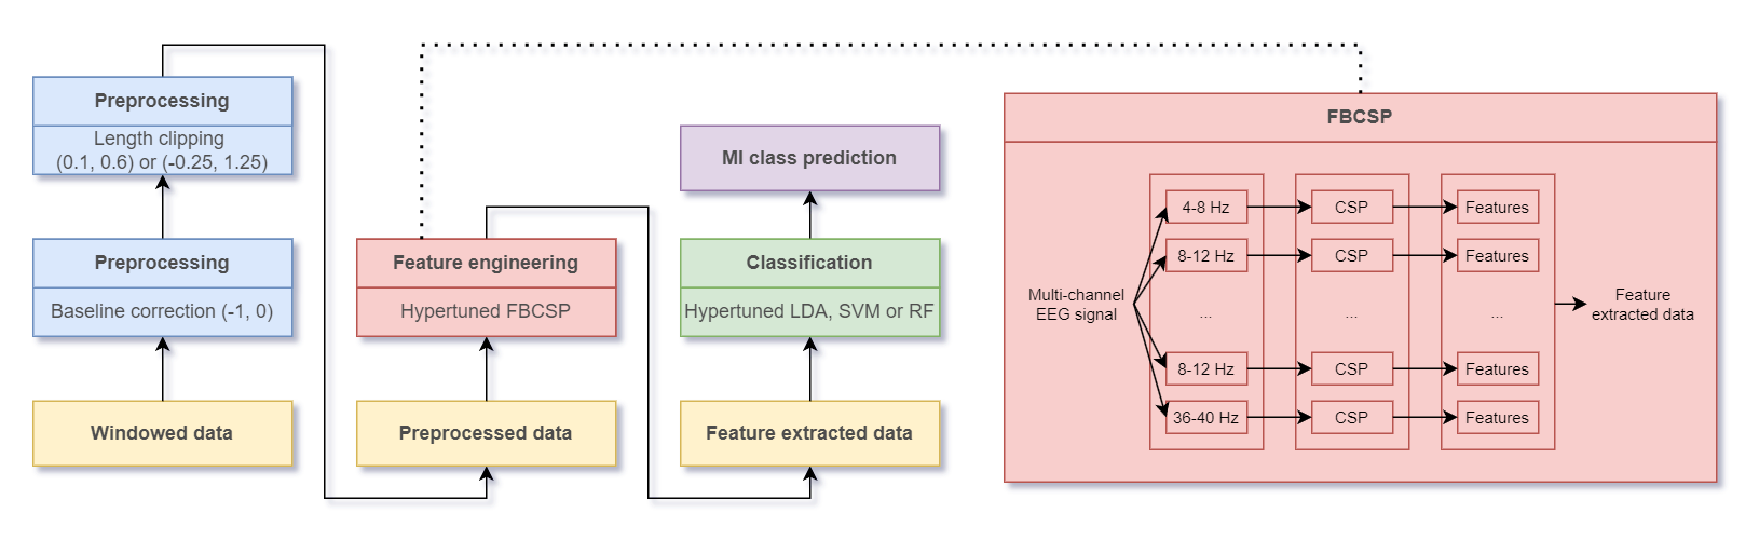
\includegraphics[width=\linewidth]{../images/offline/fbcsp_pipeline.pdf}
    \captionsetup{width=0.8\linewidth}
    \captionsetup{justification=centering}
    \caption{Visual overview of a proposed \gls{fbcsp} pipeline used for \gls{mi} \gls{eeg} using multiple traditional two-step \gls{ml} classifiers.}
    \label{fig:offline_bci_system_fbcsp_pipeline}
\end{figure}

Since the frequency band has such a significant influence on the performance of \gls{csp}, as discussed in Section \ref{subsec:offline_bci_system_two_step_ml_basic_csp_issue}, many extensions to \gls{csp} have been introduced to automate the learning of the best frequency band(s).
One popular extension to \gls{csp} that builds upon the idea of learning frequency-bands from labelled data is \gls{fbcsp} as proposed by \citet{eeg_model_fbcsp}.
Figure \ref{fig:offline_bci_system_fbcsp_pipeline} shows how a potential \gls{fbcsp} pipeline may look.
There are two main differences with the previous pipeline that was shown in Figure \ref{fig:offline_bci_system_csp_fixed_filter_pipeline}: the removal of the manual frequency filter and the replacement of \gls{csp} feature extraction by \gls{fbcsp} feature extraction.

Intuitively, \gls{fbcsp} performs multiple frequency band filters with different boundaries and stores the results on separate independent threads.
For each of those threads, traditional \gls{csp} is then performed, resulting in many different \gls{csp} features.
Since this data would likely be too complex to be handled by a traditional two-step \gls{ml} classifier, a smaller subset of features is selected from the \gls{csp} filtered signal.
The list of these final features, with multiple features per original thread, is then provided to the classifier as before.
This \gls{fbcsp} concept is also illustrated in Figure \ref{fig:offline_bci_system_fbcsp_pipeline}.
It should become clear that many different approaches for creating potentially overlapping frequency bands are possible and that the final feature extraction from the \gls{csp} transformed signals can also differ greatly.
These are all aspects that can be optimized based on the implementation of the proposed algorithm.
It should also be noted that \gls{fbcsp} does not explicitly learn frequency bands but rather provides multiple features from multiple frequency bands for which it relies on the classifier to ignore those that have no or little information.

Whilst being a relatively simple extension to \gls{csp}, \gls{fbcsp} combined with a classifier such as \gls{svm} or \gls{rf} has been proven successful at classifying \gls{mi} \gls{eeg} with far greater accuracy then the traditional \gls{csp} pipeline used in this master thesis \citep{eeg_model_fbcsp, four_class_mi_CSP_good, fbcsp_classi_eeg_mi}.
However, the implementation and evaluation of such a pipeline fall outside the scope of this master thesis.
It should also be noted that whilst \gls{fbcsp} is often used in literature it is not included in any of the popular Python \gls{eeg} processing libraries.
Providing this feature extraction method as an \gls{sklearn} compatible component can be a helpful future work to facilitate pipeline development of future research.
It is noted that some open-source Python implementations of \gls{fbcsp} are available but they have limited support and documentation \citep{fbcsp_git1, fbcsp_git2}.



% ---------------------------------------------- 
% One-step DL approaches
% ---------------------------------------------- 
\section{Convolutional-based one-step DL approaches}
\label{sec:offline_bci_system_one_step_dl}

% TODO: start here
% Figure van pipeline met component "DL classifier" zodat je nadien gewoon enkel de classifer architecture kan tonen

TODO

% - - - - - - - - - -
% EEGNet
% - - - - - - - - - -
% TODO: We gebruiken speciale dropoff, niet de "traditionele"

\subsection{EEGNet}
\label{subsec:offline_bci_system_one_step_dl_eegnet}

TODO

% - - - - - - - - - -
% DeepConvNet
% - - - - - - - - - -

\subsection{DeepConvNet}
\label{subsec:offline_bci_system_one_step_dl_deepconvnet}

TODO

% - - - - - - - - - -
% ShallowConvNet
% - - - - - - - - - -

\subsection{ShallowConvNet}
\label{subsec:offline_bci_system_one_step_dl_shallowconvnet}
% TODO: Bespreek moeilijkheid bepalen goede dropoff want heel data dependent
% TODO: heeft 2 custom objects nodig - ook bespreken
% TODO: bespreek ossilication - https://stackoverflow.com/questions/55894132/how-to-correct-unstable-loss-and-accuracy-during-training-binary-classificatio

TODO

% - - - - - - - - - -
% Interpreting 
% - - - - - - - - - -

\subsection{Interpreting these black box models}
\label{subsec:offline_bci_system_one_step_dl_interpreting}

TODO

% ---------------------------------------------- 
% Adding recurrent NN
% ---------------------------------------------- 
\section{Adding memory to one-step DL approaches}
\label{sec:offline_bci_system_adding_memory}

TODO

% cnn_bilstm_eeg_robot_arm

% - - - - - - - - - -
% time series
% - - - - - - - - - -

\subsection{Using the time series property of EEG data}
\label{subsec:offline_bci_system_adding_memory_time_series}

TODO

% - - - - - - - - - -
% LSTM eegnet
% - - - - - - - - - -

\subsection{Adding an additional LSTM layer to EEGNet}
\label{subsec:offline_bci_system_adding_memory_lstm_eegnet}

TODO

% - - - - - - - - - -
% Convolutional LSTM eegnet
% - - - - - - - - - -

\subsection{EEGNet with convolutional LSTM layer}
\label{subsec:offline_bci_system_adding_memory_convlstm_eegnet}

% Geen specifieke CUDA optim in Keras en dus trage training waardoor limited experiments

TODO

% ---------------------------------------------- 
% CONCLUSIONS OF CHAPTER
% ---------------------------------------------- 
\section{Chapter conclusions}
\label{sec:offline_bci_summary}
% TODO: summary of this chapter

TODO